% Chapter 1 (from pres-main tex file)
% New Trends in Research
% Author: Javier Reyes

\subsection{Design}

\begin{frame}
	\frametitle{Application design}
	The expected application should communicate with any of the available devices on the CAN bus of the robot. \\
	\vfill
	The CAN bus operates on a 500 kbps baud rate, with CANH-CANL voltage levels between 0-5V. % TODO: check
\end{frame}

\begin{frame}[fragile]
	\frametitle{Application design}
	Baud Rate for CAN module requires parameters tuning:
	\begin{itemize}
		\item Time Segment 1
		\item Time Segment 2
		\item Sinchronization Jump Width
		\item Baud Rate Prescaler
	\end{itemize}
	Bit timing is defined based on a subdivision value \textbf{Time Quanta}, on which all bit parameters will be measured.
	\begin{exampleblock}{CAN Baud Rate config}
		\resizebox{0.95\textwidth}{!}{%
			$freqBit\_Rate = \frac{ freqCAN\_REF\_CLK }{ \left( BAUD\_RATE\_PRESCALER + 1 \right) \cdot \left( 3 + TS1 + TS2 \right) }$%
		}
	\end{exampleblock}
\end{frame}

\begin{frame}
	\frametitle{Application design}
	After unsuccesful tests with calculated values, based on the default 100 MHz CAN\_REF\_CLK value, a web tool\footnote[frame]{See \underline{http://www.bittiming.can-wiki.info/}} for CAN parameters calculation was found.
	\vfill
	\begin{figure}
		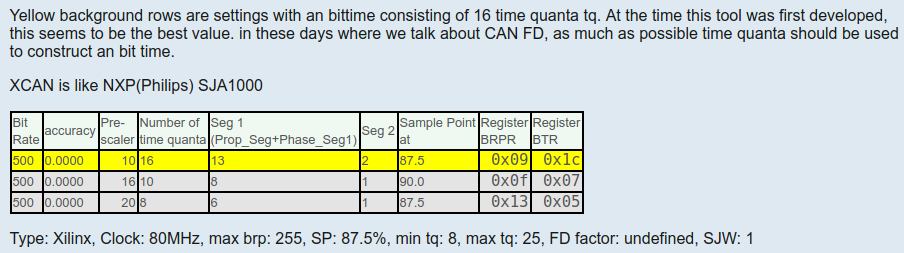
\includegraphics[width=0.9\textwidth]{can-calc.png}
		\caption{CAN bit time calculator.}\label{fig:can-calc}
	\end{figure}
\end{frame}

\begin{frame}
	\frametitle{Application design}
	The new calculation procures to obtain an integer value of TQ, which was possible setting CAN\_REF\_CLK to 80 MHz. Given the settings from the web tool, the config is coded into the application:
	\lstinputlisting[language=C, basicstyle=\tiny\ttfamily, tabsize=2, commentstyle=\color{darkgray}, keywordstyle=\color{blue}, backgroundcolor=\color{lightgray}, morekeywords={\#define}, firstline=41, lastline=56, breaklines=true, numbers=left]{../../../git/DAEbot/Devices/Zynqberry_OperatorPlus/zynqberryHW_CAN/zynqberryHW_CAN.sdk/zynqberryCAN/src/main.c}
\end{frame}

\begin{frame}
	\frametitle{Application design}
	\begin{columns}
		\begin{column}{0.5\textwidth}
			\begin{figure}
				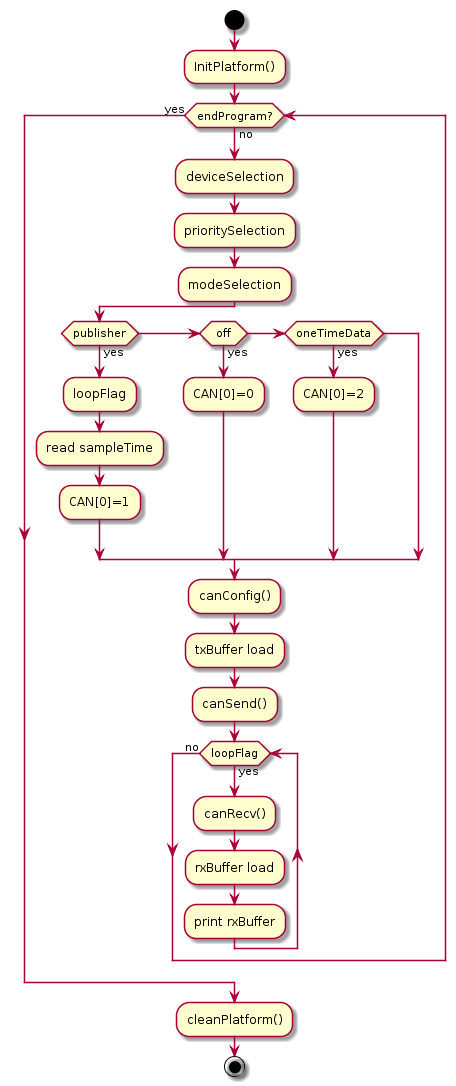
\includegraphics[width=0.45\textwidth]{activity-diag.png}
				\caption{Activity diagram.}\label{fig:activity-diag}
			\end{figure}
		\end{column}
		\begin{column}{0.5\textwidth}
			\begin{figure}
				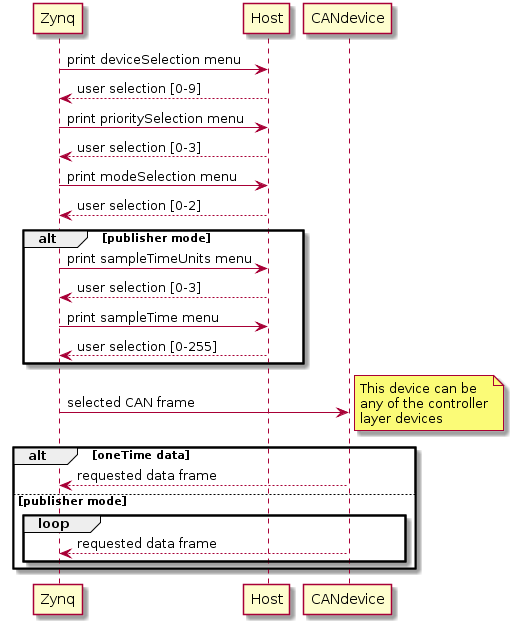
\includegraphics[width=0.8\textwidth]{sequence-diag.png}
				\caption{Sequence diagram.}\label{fig:sequence-diag}
			\end{figure}
		\end{column}
	\end{columns}
\end{frame}

\begin{frame}
	\frametitle{Application design}
	In order to enable the correct device identification on the CAN frames, the identifiers defined in the project are stored in an array available in the code. Any further new device should be included by including its identity value in the array, and adding the option in the menu.
	\vfill
	\lstinputlisting[language=C, basicstyle=\tiny\ttfamily, tabsize=2, commentstyle=\color{darkgray}, keywordstyle=\color{blue}, backgroundcolor=\color{lightgray}, morekeywords={u8}, firstline=79, lastline=91, breaklines=true, numbers=left]{../../../git/DAEbot/Devices/Zynqberry_OperatorPlus/zynqberryHW_CAN/zynqberryHW_CAN.sdk/zynqberryCAN/src/main.c}
\end{frame}

\subsection{Results}

\begin{frame}[standout]
	Thank you!
\end{frame}